\chapter[Fundamentação Teorica]{Fundamentação Teórica}
\addcontentsline{toc}{chapter}{Fundamentação Teórica}
\label{chap:teorico}

Neste capítulo, são conferidos os principais referenciais que embasam o presente trabalho, com o intuito de realizar contribuições para a área de Engenharia de \emph{Software}, especificamente ao que diz respeito as áreas de Inteligencia artificial e Segurança de dados.

O Capítulo encontra-se organizado em seções, sendo as mesmas escritas orientando-se pela literatura:
\hyperref[sec:fundamentos]{Fundamentos de Aprendizado de Máquina}, focando na contextualização do que é machine learning e seus algoritmos de treinamento tradicionais. Em sequência abordaremos o principal tópico de estudo, o tópico de \hyperref[sec:federado]{Aprendizado federado} vai tratar do surgimento desse tipo de treinamento, algumas das oportunidades e desafios que o modelo de treinamento enfrenta, ferramentas de proteção de dados associadas ao modelo, tipos de ataques e medidas de segurança em ambientes descentralizados, alguns estudos de caso e aplicações práticas e por último, desenvolvimentos tecnológicos e perspectivas futuras para o Aprendizado federado.

\section{Fundamentos de Aprendizado de Máquina}
\label{sec:fundamentos}

\subsection{Definição}

O campo do aprendizado de máquina, uma disciplina essencial dentro da inteligência artificial, tem raízes históricas profundas. A criação do termo "aprendizado de máquina" é creditado a Arthur Samuel, um pioneiro no campo, que o introduziu em 1959\cite{samuel1959}. Samuel, conhecido por suas contribuições inovadoras no desenvolvimento de programas de xadrez autônomos, formalizou o conceito como a habilidade de sistemas computacionais aprenderem automaticamente sem programação explícita. A visão de Samuel estabeleceu as bases para a revolução na interação entre máquinas e dados, antecipando a evolução de algoritmos capazes de aprimorar seu desempenho ao longo do tempo por meio da adaptação a novas informações e experiências.

Durante os anos 80 e 90, a ênfase se deslocou para modelos mais complexos, incluindo redes neurais, com pesquisadores notáveis como Geoffrey Hinton, Yann LeCun e Yoshua Bengio desempenhando papéis cruciais. Essa época marcou a adoção crescente de redes neurais profundas e técnicas de aprendizado profundo, transformando o aprendizado de máquina e inaugurando uma nova era \cite{hinton2012deep}. O campo continuou a evoluir para abranger técnicas diversas, desde aprendizado supervisionado e não supervisionado até métodos mais avançados, como aprendizado por reforço e aprendizado semi-supervisionado abordados em livros como "Deep Learning" escrito por Goodfellow \cite{goodfellow2016deep}.

A definição contemporânea de aprendizado de máquina engloba uma diversidade de técnicas que se adaptam às demandas crescentes de manipulação de grandes volumes de dados e à necessidade de extrair insights, não se limitando mais apenas a algoritmos preditivos. Além disso, lidar com problemas atuais, como ética e privacidade, mostra que é importante equilibrar a inovação com questões sociais e éticas como abordado por Floridi e Cowls\cite{floridi2018ai}.

\subsection{Algoritmos de Treinamento Tradicionais}

Algoritmos clássicos têm desempenhado um papel crucial no progresso notável alcançado em aplicações de inteligência artificial, alguns deles como o de Regressão Linear na previsão de tendências econômicas, Máquinas de Vetores de Suporte (SVM) para diagnósticos médicos para classificação de imagens, ajudando na detecção de câncer em imagens de ressonância magnética ou tomografia computadorizada, e Redes Neurais de Feedforward em sistemas de reconhecimento de fala. A robustez desses métodos reside na simplicidade conceitual e na interpretabilidade, sendo capazes de aprender padrões a partir de dados de treinamento para realizar tarefas específicas. A Regressão Linear, por exemplo, é amplamente utilizada em problemas de previsão, enquanto as SVMs têm se destacado em tarefas de classificação, e as Redes Neurais de Feedforward têm demonstrado eficácia em problemas complexos, proporcionando um entendimento mais profundo dos dados \cite{bishop2006pattern} \cite{russell2016artificial}.

Um dos desafios inerentes é a capacidade de lidar com dados não lineares de forma eficiente. Enquanto métodos como SVM podem ser estendidos para incluir kernels não lineares, a complexidade computacional muitas vezes aumenta substancialmente. Além disso, a interpretabilidade pode diminuir à medida que a complexidade do modelo aumenta, tornando difícil compreender os processos subjacentes, especialmente em redes neurais profundas \cite{goh2017deep}.

Quando se trata de privacidade de dados, esses algoritmos tradicionais enfrentam algumas dificuldades. A coleta centralizada de dados para treinamento pode comprometer a privacidade dos usuários, expondo informações sensíveis a potenciais violações de segurança. Métodos como a Regressão Logística podem ser vulneráveis a ataques de reengenharia, nos quais modelos treinados são explorados para recuperar dados originais \cite{fredrikson2014privacy}.

A constante busca por algoritmos mais eficientes e seguros destaca a importância de equilibrar os pontos fortes e fracos dessas abordagens tradicionais. À medida que avançamos, é crucial incorporar técnicas inovadoras, como o aprendizado federado e a privacidade diferencial, para superar os desafios relacionados à privacidade de dados e aprimorar a eficácia geral dos modelos de inteligência artificial.

\section{Aprendizado Federado}
\label{sec:federado}

\subsection{Definição}

O termo "Aprendizado Federado" foi introduzido por Mcmahan em 2016, marcando uma mudança paradigmática na colaboração descentralizada de modelos de inteligência artificial\cite{mcmahan2017communication}. Essa abordagem, muitas vezes referida como "Aprendizado Colaborativo", destaca-se por permitir que modelos sejam treinados localmente em dispositivos distribuídos, preservando a privacidade dos dados dos usuários enquanto contribui para um modelo global aprimorado.

Os pontos fortes do AF residem na capacidade de treinar modelos de maneira colaborativa, alavancando a diversidade de dados locais sem a necessidade de compartilhar informações sensíveis centralmente. Isso se revela especialmente valioso em cenários onde a segurança e a privacidade dos dados são prioridades, como é o caso em ambientes de saúde e finanças. A descentralização do treinamento permite que organizações colaborem efetivamente sem comprometer a confidencialidade dos dados\cite{yang2019federated}.

Quando se trata de privacidade de dados, o Aprendizado Federado enfrenta desafios singulares. Embora a descentralização do treinamento preserve a privacidade local, informações sensíveis ainda podem ser inferidas a partir dos modelos globais. Técnicas avançadas, como a aplicação de Privacidade Diferencial, tornam-se essenciais para mitigar riscos de divulgação de informações individuais durante a colaboração federada\cite{geyer2017differentially}.

É interessante explorar as complicações do AF em comparação com os métodos tradicionais de treinamento de modelos de inteligência artificial. No treinamento convencional, um modelo centralizado é alimentado com dados provenientes de diversas fontes, consolidando-os em um único local para o ajuste dos parâmetros. Esse processo, embora eficaz, levanta preocupações quanto à privacidade, segurança e eficiência, especialmente quando lidamos com dados sensíveis e distribuídos \cite{goodfellow2016deep}.

No treinamento tradicional, os dados são reunidos em um servidor central, onde o modelo é ajustado iterativamente utilizando a metodologia de otimização de gradiente descendente. Esse método, embora tenha sido a base para muitos avanços na inteligência artificial, enfrenta algumas dificuldades como a necessidade de compartilhamento massivo de dados, o que pode comprometer a privacidade do usuário. A centralização dos dados também implica em vulnerabilidades de segurança, tornando-se um ponto único de falha. Adicionalmente, o treinamento tradicional pode tornar-se computacionalmente oneroso, especialmente em grandes conjuntos de dados e modelos complexos \cite{sutskever2013importance}.

\begin{figure}[ht]
    \centering
    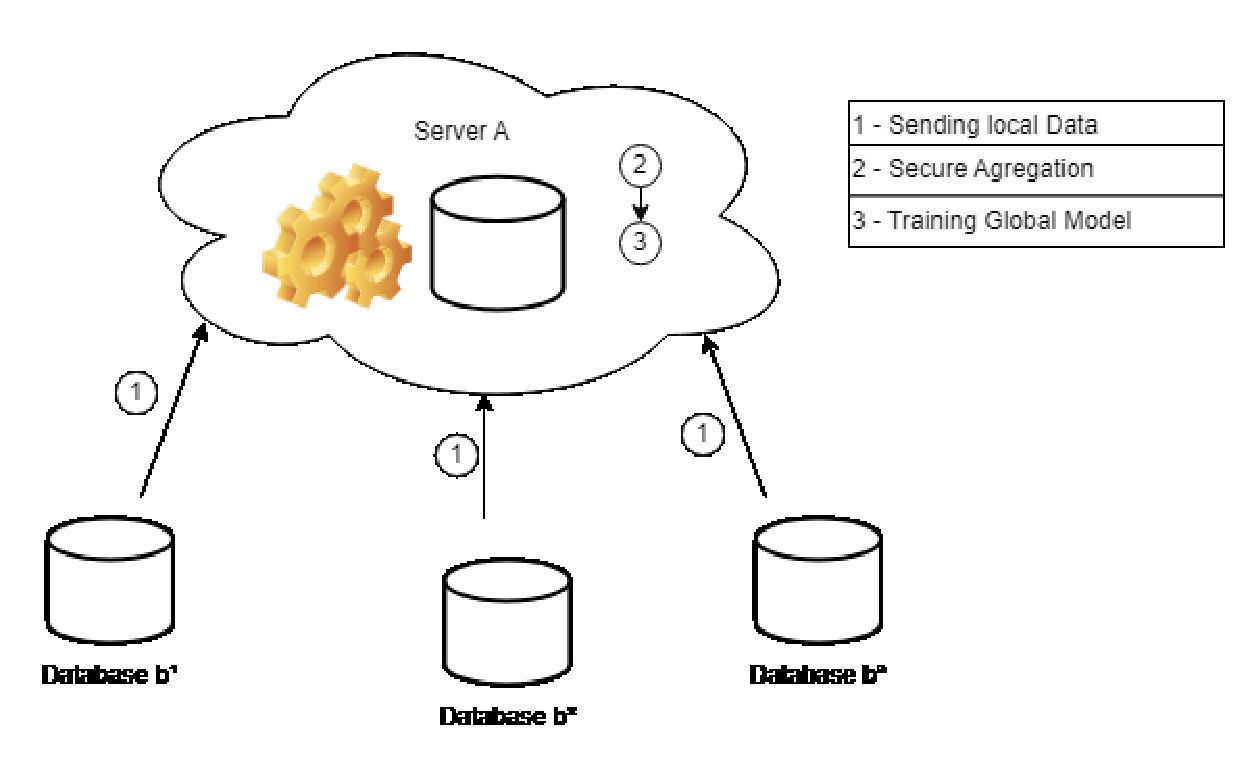
\includegraphics[scale=0.50]{figuras/teorica/centralizedDiagram.eps}
    \caption{Modelo de Treinamento Centralizado.}
    \label{fig:TraditionalCentralizedLearning}
\end{figure}

O Aprendizado Federado, por outro lado, propõe uma abordagem descentralizada e colaborativa. No contexto do AF, os modelos são treinados localmente em dispositivos distribuídos, como smartphones ou servidores locais, antes de compartilhar atualizações resumidas com um servidor central. Este, por sua vez, coordena as contribuições de todos os dispositivos para ajustar o modelo global. Esse processo de treinamento colaborativo permite a preservação da privacidade dos dados, uma vez que informações sensíveis permanecem no local de origem\cite{mcmahan2017communication}.

\begin{figure}[ht]
    \centering
    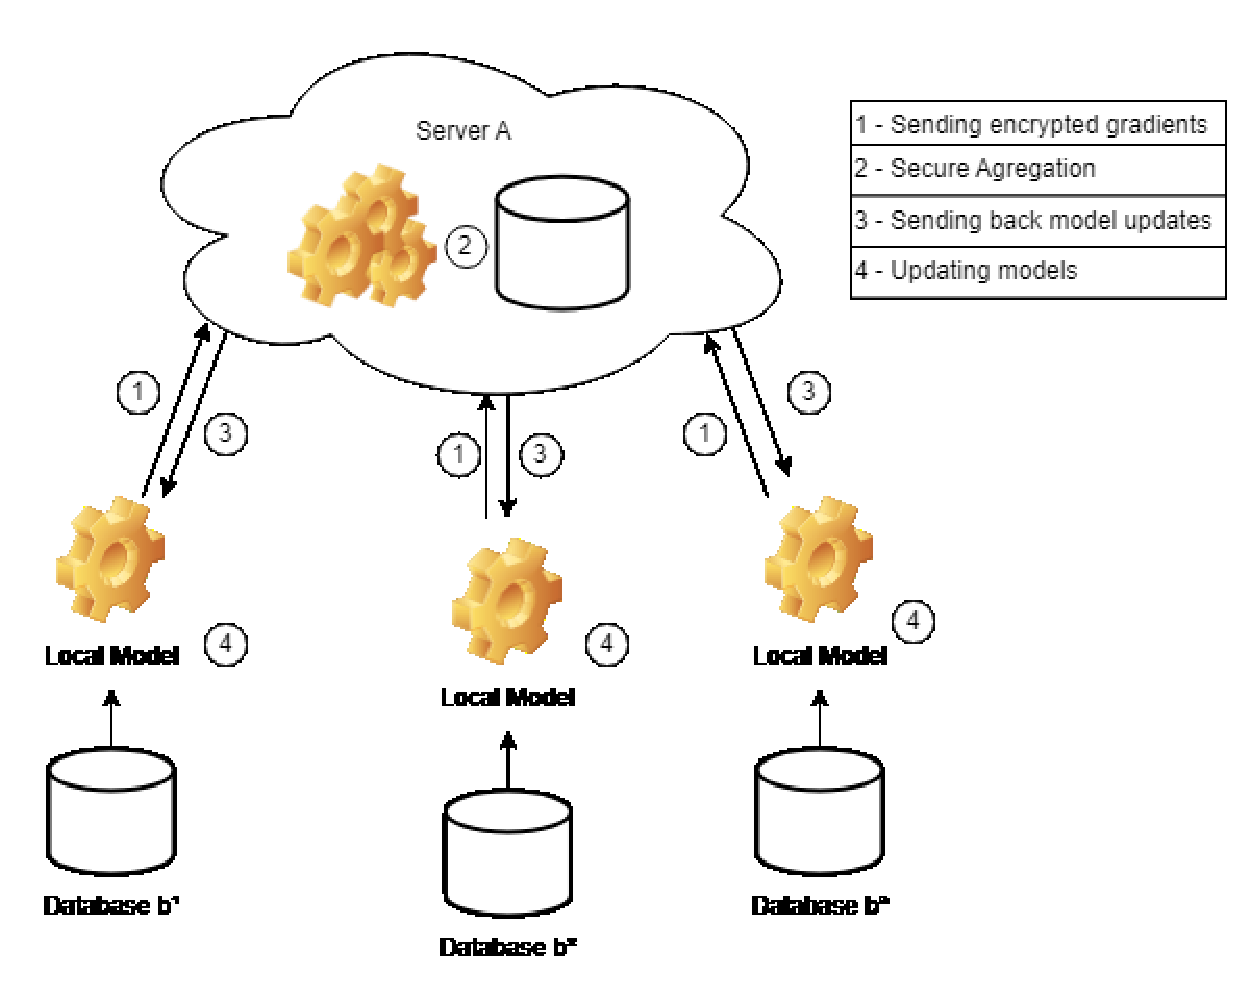
\includegraphics[scale=0.50]{figuras/teorica/federatedDiagram.eps}
    \caption{Modelo de Treinamento - Aprendizado Federado.}
    \label{fig:FederatedLearning}
\end{figure}

A eficácia do Aprendizado Federado é evidenciada pela sua capacidade de superar algumas das limitações dos métodos tradicionais. Ao descentralizar o treinamento, o AF elimina a necessidade de transferir grandes volumes de dados, facilitando a mitigação dos riscos associados à exposição de informações sensíveis. Além disso, o Aprendizado Federado oferece uma solução eficaz para a adaptação de modelos a diferentes características dos dados locais, promovendo a robustez e generalização do modelo global. A descentralização do treinamento reduz a carga computacional no servidor central, distribuindo o esforço computacional entre os dispositivos participantes\cite{yang2019federated}. Isso não apenas acelera o treinamento, mas também possibilita a utilização de dispositivos com recursos computacionais limitados, tornando o processo mais eficiente e acessível. Além disso, a abordagem federada minimiza os riscos de segurança, pois não há necessidade de transferir dados sensíveis centralmente\cite{bonawitz2019towards}.

\subsection{Oportunidades e Desafios}

O surgimento do aprendizado federado vem para aproveitar das principais fragilidades dos modelos de treinamento com dados centralizados como a capacidade de preservar a privacidade dos usuários ou a heterogeneidade dos dados. Ao permitir que o treinamento ocorra localmente em dispositivos individuais, o AF elimina a necessidade de transferir grandes volumes de dados para um servidor central, mitigando assim os riscos associados à exposição de informações sensíveis. Essa abordagem é particularmente relevante em setores como saúde e finanças, onde a confidencialidade dos dados é imperativa \cite{mcmahan2017communication}.

Além disso, o Aprendizado Federado oferece uma solução para o desafio da heterogeneidade dos dados distribuídos. Ao permitir que modelos sejam treinados em locais distintos, onde as características dos dados podem variar, o AF promove a adaptação local sem comprometer a criação de um modelo global robusto. Essa flexibilidade é crucial em cenários nos quais a diversidade de dados é uma característica intrínseca, como em aplicações urbanas ou de Internet das Coisas (IOT) \cite{yang2019federated}.

Ao descentralizar o processo de treinamento, o AF reduz a carga computacional em um servidor central, distribuindo o esforço computacional entre os dispositivos participantes. Isso não apenas acelera o treinamento, mas também possibilita a utilização de dispositivos com recursos computacionais limitados, ampliando o alcance do treinamento de modelos de inteligência artificial\cite{bonawitz2019towards}.

\subsection{Privacidade Diferencial como Ferramenta de Proteção}

Desenvolvida para proteger informações sensíveis durante o processamento de dados, a Privacidade Diferencial (DP) oferece uma abordagem robusta e matematicamente fundamentada para garantir a confidencialidade dos dados individuais \cite{dwork2011}. A Privacidade Diferencial baseia-se no princípio de adicionar ruído controlado aos resultados de consultas realizadas em um banco de dados. Esse ruído introduzido protege a privacidade individual, tornando difícil discernir a contribuição específica de um único dado no conjunto. Formalmente, um mecanismo é diferencialmente privado se, para qualquer dois conjuntos de dados que diferem apenas em um elemento, a probabilidade de obter o mesmo resultado permanece próxima, mesmo que seja revelado o resultado da consulta \cite{dwork2011}.

No cenário do AF, a integração da Privacidade Diferencial é essencial para assegurar a confidencialidade dos dados contribuídos por dispositivos locais. O processo de treinamento federado envolve a colaboração de modelos locais em dispositivos distribuídos, mas a agregação dessas informações pode expor informações sensíveis. Ao aplicar mecanismos de DP durante a agregação, cada dispositivo contribui diferencialmente para o modelo global, mitigando riscos de divulgação de dados individuais\cite{abadi2016}.

Para ilustrar a eficácia da Privacidade Diferencial no treinamento federado, consideremos o exemplo de um sistema de recomendação personalizada. Ao incorporar técnicas de DP na agregação de preferências locais dos usuários, o sistema pode aprender padrões de comportamento de forma coletiva sem expor escolhas individuais. Da mesma forma, em diagnósticos médicos distribuídos, a aplicação de DP assegura que os modelos federados aprendam com imagens sem revelar informações específicas de pacientes, promovendo avanços na pesquisa médica colaborativa\cite{shokri2015}.

\subsection{Ataques e medidas de Segurança em Ambientes Descentralizados}

Embora o AF ofereça uma solução promissora para a preservação da privacidade dos dados, ele também enfrenta ameaças consideráveis provenientes de ataques sofisticados. A compreensão desses desafios é essencial para avançar em direção a modelos mais seguros e robustos\cite{geyer2017differentially}. Alguns dos ataques mais comuns utilizados contra os modelos de treinamento descentralizados são os:

\begin{itemize}
    \item Ataques de Inversão de Modelo
    \item Ataques de Envenenamento de Dados
    \item Ataques de Inferência Estatística
\end{itemize}

\subsubsection{Ataques de Inversão de Modelo}

Um dos principais desafios de segurança em modelos descentralizados é representado pelos ataques de inversão de modelo. Nestes ataques, um adversário tenta inferir informações sensíveis sobre os dados de treinamento a partir do modelo global treinado. Essa técnica pode ser particularmente eficaz quando o modelo é treinado em dados sensíveis, como informações médicas ou financeiras. Estratégias avançadas, como a reconstrução do conjunto de treinamento original, podem ser empregadas para recuperar detalhes específicos, comprometendo assim a privacidade dos dados\cite{fredrikson2014privacy}. Para mitigar os ataques de inversão de modelo em treinamentos descentralizados, estratégias como \textbf{limitação de informações no modelo global} (Reduzir a quantidade de informações específicas incorporadas no modelo global pode minimizar o risco de ataques) e \textbf{Controle de acessos}, podem ser utilizadas.

\subsubsection{Ataques de Envenenamento de Dados}

Outra classe crítica de ataques em modelos descentralizados é representada pelos ataques de envenenamento de dados. Nestes cenários, um adversário introduz intencionalmente dados maliciosos no conjunto de treinamento distribuído, visando manipular o modelo global resultante. Esses ataques podem levar a decisões incorretas do modelo e comprometer sua utilidade e confiabilidade. Estratégias de defesa, como \textbf{detecção de dados envenenados} e \textbf{técnicas de aprendizado robusto}, tornam-se essenciais para mitigar esses riscos\cite{bagdasaryan2018backdoor}.

\subsubsection{Ataques de Inferência Estatística}

Além disso, modelos de treinamento descentralizados estão sujeitos a ataques de inferência estatística, nos quais adversários tentam deduzir informações sensíveis explorando padrões estatísticos nos modelos ou nas atualizações de parâmetros. Esses ataques podem revelar informações sobre os dados de treinamento local, mesmo sem acesso direto a eles. Técnicas como \textbf{Privacidade Diferencial} têm sido propostas para mitigar essas ameaças, introduzindo ruídos controlados nas atualizações de modelo tornando mais difícil para um atacante inferir informações específicas sobre os dados locais\cite{shokri2015privacy}.

\subsection{Estudos de Caso e Aplicações Práticas}

O crescente volume de dados e a necessidade de preservar a privacidade dos usuários impulsionaram o desenvolvimento do Aprendizado Federado como uma abordagem no treinamento de modelos de Inteligência Artificial em ambientes descentralizados. Diversos estudos de caso destacam o sucesso do AF em diferentes contextos. Em um desses casos, a aplicação do AF na área de saúde permitiu o treinamento de modelos de diagnóstico em dados distribuídos entre várias instituições médicas, preservando informações sensíveis dos pacientes \cite{smith2018privacy}. Em outro cenário, empresas financeiras adotaram o AF para a detecção de fraudes, permitindo a colaboração entre instituições sem a necessidade de compartilhar detalhes específicos de transações individuais\cite{jones2020federated}.

Outro estudo de caso na área de educação revela como o AF está transformando o cenário educacional. Em uma colaboração entre instituições acadêmicas, o modelo de treinamento foi implementado para aprimorar a personalização do ensino sem comprometer a privacidade dos estudantes \cite{edutechcollab2020}. Os modelos de IA treinados localmente em diferentes escolas foram agregados de forma segura, permitindo que os educadores recebessem insights valiosos sobre o desempenho dos alunos, adaptando estratégias de ensino de maneira eficaz. Esse estudo não apenas demonstrou a eficácia do AF na área educacional, mas também destacou sua capacidade de superar desafios específicos relacionados à privacidade e à diversidade dos dados.

Além dos setores tradicionais, o Aprendizado Federado tem se destacado na promoção da colaboração científica. Em um estudo colaborativo entre instituições de pesquisa em diferentes países, o AF foi utilizado para treinar modelos de predição em conjuntos de dados descentralizados, envolvendo pesquisadores em diversas disciplinas \cite{scicollab2021}. O estudo evidenciou não apenas a aplicabilidade do AF em ambientes científicos, mas também seu potencial para integrar especialidades diversas, impulsionando descobertas e avanços mais amplos na pesquisa.

Resultados obtidos em projetos relevantes reforçam a eficácia do AF. Uma pesquisa acadêmica conduzida por especialistas em privacidade e IA demonstrou que a implementação do AF em plataformas de redes sociais possibilitou a personalização de recomendações de conteúdo sem comprometer a privacidade dos usuários \cite{privacyintech2022}. Em um projeto colaborativo entre instituições de pesquisa e empresas do setor de energia, o AF facilitou a previsão de demanda de forma descentralizada, garantindo a confidencialidade dos dados operacionais \cite{energytechcollab2019}.

A revisão desses estudos de caso destaca a versatilidade do AF e sua aplicabilidade em diversos setores. A capacidade de treinar modelos de IA em dados descentralizados, preservando a privacidade dos usuários, é um marco na busca por soluções éticas e eficientes. Esses casos oferecem insights valiosos para pesquisadores, profissionais e gestores que buscam adotar o AF em suas práticas, promovendo uma abordagem mais colaborativa e segura no avanço da IA.

\subsection{Perspectivas Futuras e Desenvolvimentos Tecnológicos}

Uma tendência emergente crucial é a busca pela otimização do processo federado, visando aprimorar a eficiência e a eficácia do treinamento. A introdução de algoritmos de otimização mais avançados, como algoritmos federados de segunda ordem, tem o potencial de acelerar a convergência do treinamento, reduzindo a carga computacional nos dispositivos participantes e, consequentemente, promovendo uma maior adesão ao modelo federado \cite{konecny2016federated}.

Outra tendência que ganha destaque é a aplicação do AF em cenários de aprendizado contínuo e online. Com o crescente volume de dados gerados em tempo real, o AF está sendo adaptado para suportar treinamento incremental, permitindo que modelos federados evoluam continuamente à medida que novos dados são incorporados. Essa abordagem é particularmente relevante em ambientes como a Internet das Coisas (IoT), onde a natureza dinâmica dos dados demanda modelos de IA que possam se adaptar rapidamente às mudanças nas condições operacionais \cite{mohassel2017secureml}.

A evolução do AF não ocorre isoladamente, ela está intrinsecamente ligada ao progresso de tecnologias emergentes. O advento da computação quântica é uma área que pode revolucionar o treinamento federado. Algoritmos quânticos prometem realizar cálculos de forma exponencialmente mais eficiente do que os algoritmos clássicos, potencialmente reduzindo significativamente o tempo necessário para treinar modelos federados complexos \cite{aaronson2016read}.

A segurança no AF é uma consideração crítica e as tecnologias emergentes no campo da segurança cibernética também desempenharão um papel fundamental. A aplicação de técnicas de criptografia pós-quântica pode fortalecer ainda mais a segurança do AF, garantindo a confidencialidade dos modelos e dados distribuídos. Essa combinação de AF e criptografia pós-quântica pode proporcionar um ambiente de treinamento mais robusto em face de ameaças potenciais \cite{giovanni2020postquantum}.